\clearpage
\section{Controlador PI con Predictor Smith}
Se plantea un proceso con un retardo de la forma:

\[
  H(s) = \frac{K e^{-\theta s}}{s\tau + 1}
\]

Si el retardo es dominante, el diseño de un contrplador adecuado se vuelve muy complejo.

\begin{itemize}
    \item \textbf{$R < 0.2$ (Dominante por Capacitancia):} El tiempo muerto es despreciable. Un controlador PI o PID estándar puede sintonizarse con alta agresividad sin comprometer el margen de fase.
    \item \textbf{$0.2 \leq R < 0.5$ (Región Intermedia):} El retardo es significativo. El PID tradicional aún es capaz de controlar el proceso, pero requiere métodos de sintonía conservadores (como Cohen-Coon) que reducen la ganancia proporcional para mantener la estabilidad, sacrificando velocidad de respuesta.
    \item \textbf{$R \geq 0.5$ a $R > 1$ (Dominante por Tiempo Muerto):} Es en esta región donde se justifica la implementación del \textbf{Predictor de Smith}. 
\end{itemize}

\subsection{El Problema de la Inestabilidad}
Físicamente, cuando $t_d > \tau$, el controlador percibe un error prolongado debido al retardo de transporte y reacciona sobre-inyectando acción integral a la variable manipulada. Matemáticamente, el término $e^{-t_d s}$ introduce un desfase negativo que crece linealmente con la frecuencia ($\phi = -\omega t_d$), reduciendo drásticamente el Margen de Fase del sistema en lazo cerrado hasta cruzar el punto crítico de $-180^\circ$, causando inestabilidad.

\subsection{La Solución del Predictor}

El predictor smith parte desde la premisa de predecir la respuesta del sistema antes de que este ocurra, esto se logra mediante la obtención de un módelo matemático de la planta.

\begin{figure}[H]
  \begin{center}
    \includegraphics[width=0.8\textwidth]{figures/PS.png}
  \end{center}
  \caption{}\label{psbloques}
\end{figure}

Analizando el álgebra de bloques de la figura \ref{psbloques} con $w = 0$ se tiene.

\[
  y(s) = G_pe^{-\theta s}u(s) 
\]

\[
  u(s) = G_c e_2 = G_c(e_1 - \hat{b}(1 - e^{-\theta_m s}))
\]

\[
  u(s) = G_c(e_1 - G_c G_m u(s)(1 - e^{-\theta_m s}))
\]
\[
  u(s) = \frac{G_c e_1 }{1 + G_c G_m - G_c G_m e^{-\theta_m s}} 
\]


\[
  y(s) = G_pe^{-\theta s}(\frac{G_c e_1 }{1 + G_c G_m - G_c G_m e^{-\theta_m s}})
\]

\[
  y(s)(1 + (\frac{G_c G_p e^{-\theta s}}{1 + G_c G_m - G_c G_m e^{-\theta_m s}})) = sp (\frac{G_cG_pe^{-\theta s}}{1 + G_c G_m - G_c G_m e^{-\theta_m s}})
\]


\[
  y(s) = sp (\frac{G_c G_p e^{-\theta s}}{1 + G_c G_m - G_c G_m e^{-\theta_m s} + G_cG_pe^{-\theta s}})
\]
Finalmente

\begin{equation}
  H_{ps} = \frac{G_c(s) G_p(s) e^{-\theta s}}{1 + G_c(s) G_p(s) + G_c(s)\left[ G_m(s) e^{-\theta_m s} - G_p(s) e^{-\theta s} \right]}
  \label{psfin}
\end{equation}

Luego, asumiendo que el modelo de la planta es igual a la planta se puede decir:

\[
  G_me^{-\theta_m s} = G_pe^{-\theta s} \implies H_{ps} = \frac{G_c(s) G_p(s) e^{\theta s}}{1 + G_c(s)G_p(s)}
\]

Así logra el predictor smith dar feedback al controlador del proceso sin tener que esperar a que ocurra en la planta, lo cual permite que el controlador llegue a estado estacionario y no genera un windup integral al acumular error debido al gran retardo del sistema.

\subsection{Discretización y obtención de PI + PS}

Tomando el diagrama discreto de un predictor smith, se debe encontrar un $G_c$ tal que el controlador se comporte como un controlador como un controlador con controlador smith.

\begin{figure}[H]
  \begin{center}
    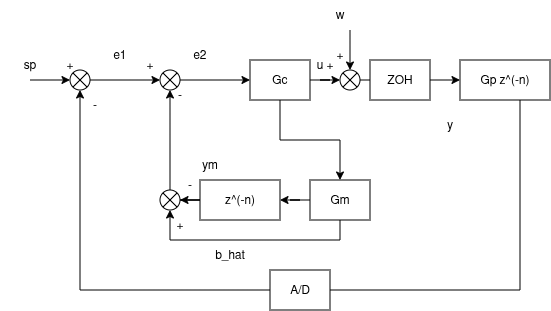
\includegraphics[width=0.8\textwidth]{figures/psz.png}
  \end{center}
  \caption{Controlador smith discreto}\label{psz}
\end{figure}

      
\[
  u(z^{-1}) = G_c(z^{-1}) e_2(z^{-1}) = G_c(z^{-1})(e_1(z^{-1}) - \hat{b}(1 - z^{-N})))
\]

\[
  u(z^{-1}) = G_c(z^{-1})(e_1(z^{-1}) - u(z^{-1})G_m(z^{-1})(1 - z^{-N})))
\]

\[
  u(z^{-1})(1 + G_c(z^{-1})G_m(z^{-1})(1 - z^{-N}))) = G_c(z^{-1})(e_1(z^{-1}))
\]

Y así finalmente, la ecuación del controaldor del predictor smith es:
\begin{equation}
  \frac{u(z^{-1})}{e_1(z^{-1})} = \frac{G_c(z^{-1})}{1 + G_c(z^{-1})G_m(z^{-1}) -G_c(z^{-1})G_m(z^{-1})z^{-N}}
\end{equation}

\subsubsection{Análisis de $y_m$ y $\hat{b}$ para el Predictor de Smith}

Para implementar el Predictor de Smith en un procesador digital, no se debe agrupar la planta y el controlador en una única ecuación en diferencias, ya que esto generaría un lazo algebraico irresoluble en tiempo de ejecución. En su lugar, el problema se divide de forma algorítmica calculando secuencialmente el modelo con retardo ($y_m$), el modelo sin retardo ($\hat{b}$), y finalmente corrigiendo el error que alimenta al controlador PI.

Asumiendo un modelo de primer orden discretizado de la forma $G_m(z^{-1}) = \frac{\beta z^{-1}}{1 - \alpha z^{-1}}$ y un tiempo muerto equivalente a $N$ muestras, el desarrollo es el siguiente:

\textbf{Análisis de $y_m$ (Predicción con retardo)}

Partimos de la función de transferencia del modelo incluyendo el tiempo muerto:
\[
  y_m(z^{-1}) = z^{-N}G_m(z^{-1})u(z^{-1})
\]
\[
  y_m(z^{-1}) = \frac{\beta z^{-(N+1)}}{1 - \alpha z^{-1}}u(z^{-1})
\]
Multiplicando de forma cruzada para despejar el denominador:
\[
  y_m(z^{-1})(1 - \alpha z^{-1}) = u(z^{-1})(\beta z^{-(N+1)})
\]
\[
  y_m(z^{-1}) - \alpha y_m(z^{-1})z^{-1} = \beta u(z^{-1})z^{-(N+1)}
\]
Aplicando la transformada $\mathcal{Z}$ inversa, obtenemos la ecuación de diferencias para la predicción con retardo:
\[
  y_m[k] = \alpha y_m[k-1] + \beta u[k-(N+1)]
\]
 
\textbf{Análisis de $\hat{b}$ (Predicción pura sin retardo)}

El predictor puro corresponde al modelo de la planta sin el tiempo muerto extra $z^{-N}$:
\[
  \hat{b}(z^{-1}) = G_m(z^{-1})u(z^{-1})
\]
\[
  \hat{b}(z^{-1}) = \frac{\beta z^{-1}}{1 - \alpha z^{-1}}u(z^{-1})
\]
Despejando de manera análoga al caso anterior:
\[
  \hat{b}(z^{-1})(1 - \alpha z^{-1}) = u(z^{-1})(\beta z^{-1})
\]
\[
  \hat{b}(z^{-1}) - \alpha \hat{b}(z^{-1})z^{-1} = \beta u(z^{-1})z^{-1}
\]
Llevando la expresión al dominio discreto $k$, la ecuación de diferencias resulta:
\[
  \hat{b}[k] = \alpha \hat{b}[k-1] + \beta u[k-1]
\]

\textbf{Cálculo del Error Modificado y Ley de Control PI}

Una vez calculadas ambas predicciones en el instante actual $k$, el algoritmo del Predictor de Smith corrige el error tradicional ($e_1[k] = SP[k] - PV[k]$) restando el efecto del modelo puro y sumando el modelo con retardo. Esto se define como el error modificado $e_2[k]$:
\[
  e_2[k] = (SP[k] - PV[k]) - \hat{b}[k] + y_m[k]
\]

Finalmente, este error modificado $e_2[k]$ es el que alimenta la ecuación en diferencias del controlador PI en su forma de velocidad (incremental):
\[
  u(z^{-1})(1 - z^{-1}) = e_2(z^{-1})(q_0 + q_1z^{-1})
\]
\[
  u(z^{-1}) - u(z^{-1})z^{-1} = q_0 e_2(z^{-1}) + q_1 e_2(z^{-1})z^{-1}
\]
Lo que se traduce en la siguiente ley de control final a ser ejecutada por el PLC:
\[
  u[k] = u[k-1] + q_0 e_2[k] + q_1 e_2[k-1]
\]

De esta manera, el controlador calcula el esfuerzo de control $u[k]$ en función de un error compensado iterativamente, eliminando el retardo de la ecuación característica del sistema sin comprometer la causalidad del código.
